\section{Flow Scheduling for Storage on the Cloud}
\label{sec:flow_scheduling}

In this section, we describe the concept of flow scheduling and then explain how we model the assignment cost based on the penalty of violating flow demand.
We also introduce how to encode the scheduling problem as a min-cost flow problem.

\subsection{Concept of Data Flow}
\label{sec:flow_rate}

A MapReduce job includes several map and reduce tasks, and each of them (on a computing facility) reads data, processes data and writes data.
The data flow rate is the size of data that goes through a facility per unit time.
For example, the processing flow rate is how fast a machine can process data, and a faster processing rate also suggests higher system throughput.
In a decoupled model, all of the read and write operations involve network activities, which can be costly and decrease the processing flow rate.
Therefore, our flow scheduling tries to maximize processing flow rate on computing facilities so that the system throughput can be increased.

The idea of flow scheduling is similar to the water treatment system.
Water supply to a desired end-user must go through several processing steps before water is delivered to users.
Users may complain if water supply is not fast enough.
This situation can happen if water supply is scarce or if the intermediate facilities cannot process water quickly or if the pipeline is not large enough or if too many users request water at the same time.
Thus, to meet the demand from users, a water treatment system should satisfy the above conditions as mush as possible.
This analogy truly reflects those factors that affect the system throughout in a decoupled Hadoop model: ensuring the quality of data supply and the flow rate of data processing can increase the system throughput.
More precisely, if the flow demand of a task cannot be satisfied by facilities, the scheduling decision is considered costly.

Flow rate is defined as how fast a machine can process data  or a network can transfer data.  
\begin{equation*} \label{eq:flow_rate}
R=\frac{D}{T}
\end{equation*}
Here, $D$ is the size of data and $T$ is the total time to process or transfer the data.
Throughput this paper, we use \textit{second} for the time unit and \textit{mega bytes} for the data size unit.

\textbf{Flow capability of facilities}:
We define three types of flow capability which are read, write and process.
Read flow capability is the maximum flow rate that a facility can pull data from other facilities and write flow capability is similar but its the maximum flow rate that can push data to other facilities.
The process flow capability is defined by how fast a facility can process data.
Facilities can be classified as computing nodes, storage nodes and network infrastructure.
$R^{s}_{in}$ is the read flow capability of the storage node and $R^{s}_{out}$ is the write one; similarly, $R^{n}_{in}$ and $R^{n}_{out}$ are for network infrastructure, and the computing node uses $R^{c}_{in}$ and $R^{c}_{out}$ for read and write capability.
Besides, only the computing node has the process flow capability, $R^{c}_{p}$.

\textbf{Flow demand of tasks}:
The flow demand describes the characteristic of tasks and can be used to classify tasks into CPU-intensive (low flow demand) and network-intensive (high flow demand) tasks.
A flow rate can vary during task execution, and we assume the flow rate is relatively stable, which can be reasonable because either a map task or a reduce task repeats a piece of the same code based on key-value pairs.
The $R^{t}_{in}$ and $R^{t}_{out}$ are the read and write flow demand of tasks.

\subsection{Cost Model}
\label{sec:cost_model}

In this section, we describe how to model the cost of task assignment.
The decoupled model can be model as $\{C, S, I\}$, where $C$ is the set of computing facilities, $S$ is the set of storage facilities and $I$ is the network infrastructure. 
Let $c_{i} \in C$, $s_{i} \in S$, where $i$ is an integer.
The flow capability of facilities is defined as, for example, $R^{c_{i}}_{p}$ for the processing capability on the computing node $i$ and $R^{s_{i}}_{out}$ for the write capability on the storage node $i$.
Let $r^{c}_{p}$ be the processing flow rate on a computing facility.
When $r^{c}_{p}$ approaches to $R^{c}_{p}$, the system throughput is considered increasing.
The tasks to be scheduled are $t_{ij}$, where $i$ is the \textit{ith} job in the system and $j$ is the \textit{jth} task of the job.
Similar to flow capability, $R^{t_{ij}}_{in}$ and $R^{t_{ij}}_{out}$ are the read and write flow demand of tasks.

A scheduling problem is to assign $T=\{t_{ij}\}$ to $C=\{c_{n}\}$, and our flow scheduling tries to minimize the assignment cost based on the flow rate.
Given a task, the cost of an assignment can be defined as the penalty cost that facilities cannot satisfy the flow demand of the task.
To fulfill the flow demand of tasks, we should ensure quality flow supply and quality processing flow.
There are two conditions in which an assignment can occur high penalty cost:
1) a storage facility is overloaded when $\sum_{t_{ij} \in s_i} R^{t_ij}_{in}$ is high, especially when it exceeds $R^{s_{i}}_{out}$
and
2) a computing facility is filled with network-intensive jobs, which means $\sum_{t_{ij} \in c_i} {R^{t_ij}_{in}}$ is high.

To assign a map task $t_{ij}$, suppose the input data stores on $s_n$, the cost to assign the task on $c_n$ is the sum of
\begin{equation*}
R^{t_{ij}}_{in} \times (1+\frac{r^{s_n}_{out}}{R^{s_n}_{out}}+f_{c})
\end{equation*}
and
\begin{equation*}
R^{t_{ij}}_{in} \times (1+e_{m}),
\end{equation*}
where $f_{c}$ is the parameter if $s_n$ and $c_m$ is not in the same rack, and $e_{m}$ is the effective load on $c_m$.
The effective load can be defined as $\sum_{t_{ij} \in c_m} {R^{t_ij}_{in}} - stdev(R^{t_ij}_{in})$.
If flow demands of tasks are diverse on a computing facility, we consider the assignment cost lower because overlapping CPU-intensive and network-intensive tasks can utilize resource efficiently.

When $t_{ij}$ is a reduce task, it usually reads data from multiple computing facilities; thus, we need to count all of these read cost.
Suppose $t_{ij}$ is assigned to $c_{m}$ and the reduce task need to read data from other computing facilities $c_k$, the total read cost is

\begin{equation*}
\sum_{c_{k}} R^{t_{ij}}_{in} \times (1+\frac{r^{c_k}_{out}}{R^{c_k}_{out}}+f_{c}),
\end{equation*}

where $f_c$ has the definition similar to the one above.
If $c_m$ and $c_k$ are the same node, the parameter is zero, and otherwise, the parameter is small for in-rack communication and large for cross-rack data transfer.


\begin{figure}[ht]
    \centering
    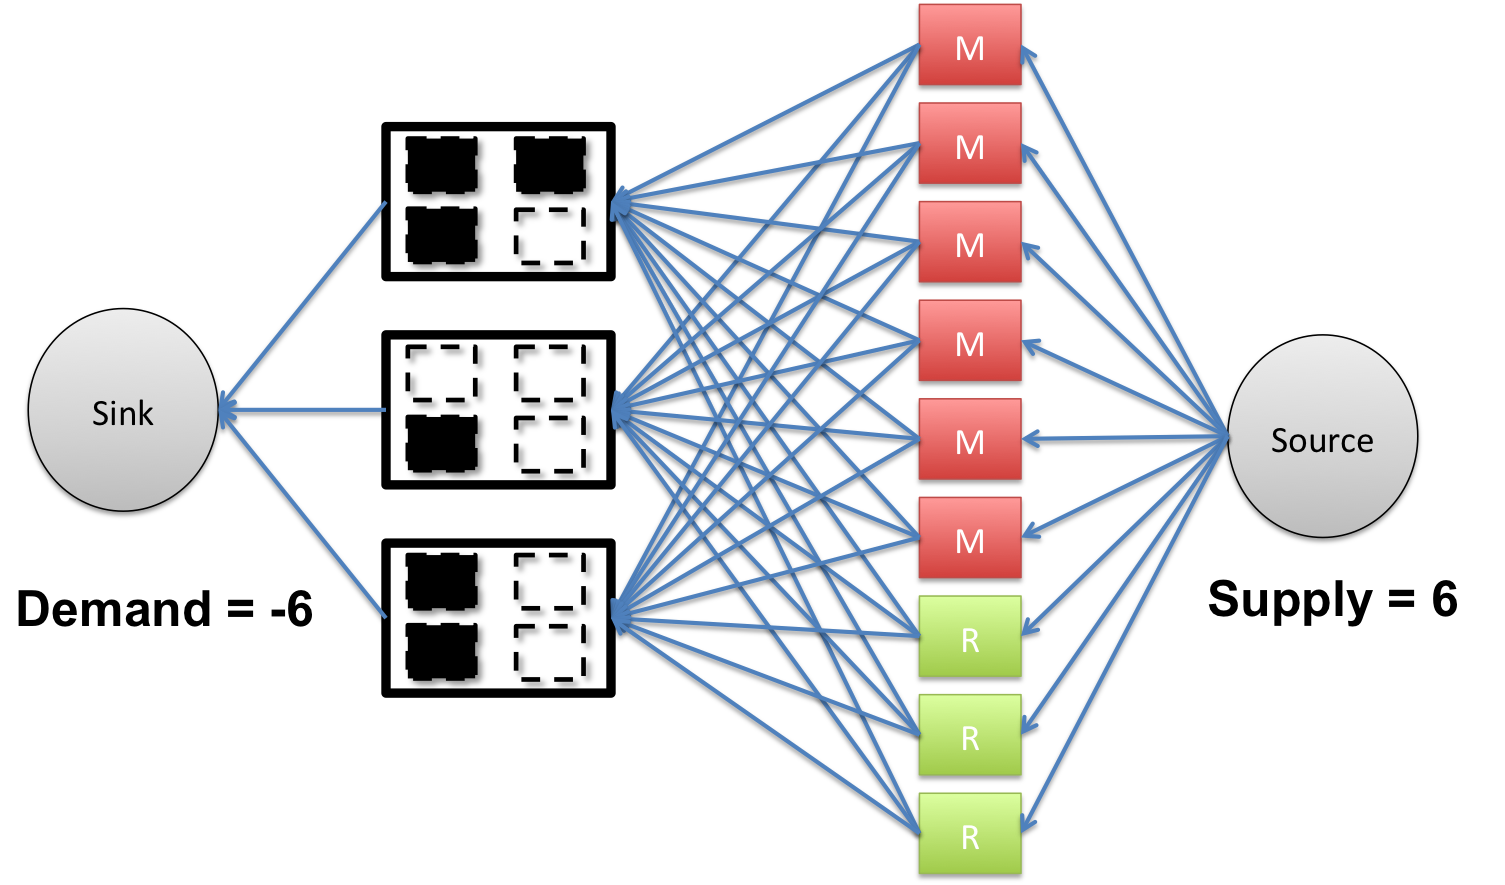
\includegraphics[width=0.8\textwidth]{figures/min_cost_model.png}
    \caption{Flow scheduling uses the penalty cost to build the min-cost flow network. The number of supply means the number of tasks to be scheduled.}
    \label{fig:min_cost_model}
\end{figure}


\subsection{Min-cost flow optimization}
\label{sec:min_cost_flow}

We argued that maximizing the processing flow rate can increase the system throughput.
As described in Section \ref{sec:cost_model}, we model the cost of task assignments as the penalty of violating flow demand.
Given the cost model, we encode the scheduling problem as a min-cost flow optimization problem.
The min-cost flow problem is a network optimization problem that looks for the cheapest way to allow a certain amount of flow through a network.
Given the flow demand of map and reduce tasks, we can decide the best path of network flow with minimum penalty cost.
For example, our flow scheduling avoids to assign a task to facilities if the flow capability of the facilities can not meet the flow demand of the tasks.
Figure \ref{fig:min_cost_model} depicts how to encode the scheduling problem to a min-cost flow problem.

The min-cost flow problem can be stated as follows:

\begin{equation*}
Minimize \; z(x)=\sum\limits_{(i,j) \in A} c_{ij}x_{ij}
\end{equation*}

subject to

\begin{equation*}
\sum\limits_{j:(i,j) \in A} x_{ij} - \sum\limits_{j:(j,i) \in A} x_{ji} = b(i) \; \forall i \in N
\end{equation*}

\begin{equation*}
0 \le x_{ij} \le u_{ij} \; \forall (i,j) \in A
\end{equation*}

In this equation, $N=\{T_{ij}, C_{k}, source, sink\}$ and the source node produces flow of capacity $n$, which is the number of available slots on computing facilities and the sink node has the flow of capability $-n$.
Each arc from $T_{ij}$ to $C_{k}$ has the cost that is defined in Section \ref{sec:cost_model}, and each arc has a lower capacity zero and a upper capacity one.
On the other had, the lower capacity and higher capacity of the arc from the source to $T_{ij}$ are both $one$, and them of the arc from $C_{k}$ to the sink are the number of available slots on $C_{k}$.
After encoding the scheduling problem, we then solve the min-cost flow problem to decide the optimal task assignment.

\section{Flow Scheduler for Hadoop}
\label{sec:flow_scheduler}

Hadoop supports pluggable resource schedulers that makes developing the flow scheduler not being a difficult challenge.
\subsection{System Architecture}
Our flow scheduler requires job profile (flow demand of tasks) and machine profile (flow capability of facilities).
Besides, we use a database to keep track of resource allocation so that next time we can understand the flow rate on facilities.
The flow scheduler runs upon AppMaster requests resources or periodically, e.g. every 5 second.
In each run, it calculate the penalty cost based on flow demand of tasks and flow capability of facilities, and then encodes the scheduling problem as stated in Section \ref{sec:min_cost_flow}.
After building the cost mode, we use the scaling push-relabled method as described in \cite{GoldbergA1997_Scaling} and their solver program to derive the optimal task assignment.

\subsection{Estimating Flow Rate}
In this section, we describe how to estimate the flow demand of tasks and flow capability of facilities.
Basically, we overload facilities to get flow capability and run a single task to derive the flow demand.
First, we measure $R^{c}_{out}$ of storage nodes to get the flow rate that a storage node can supply.
We create a NoComputation map task that only reads input data, but does not do computation and does not generate output.
We execute enough NoComputation map tasks at the same time to ensure that the out-bound bandwidth of a storage node is saturated.
The result shows that $R^{cap}_{out}$ of storage nodes is roughly close to 65\% of the theoretical network bandwidth.
Similarly, $R^{s}_{in}$  is close to $R^{s}_{out}$; therefore, we use the same number.
Regarding the flow capability of network infrastructure, we use the same number with that of storage nodes.
This is true for node communication in the same rack; however, the cross-race communication can be limited by aggregate bandwidth available at top-of-rack switches.
The real bandwidth of cross-bandwidth is hard to measure and monitor, and instead, we increase the cost of cross-rack communication in our cost model as described in \ref{sec:min_cost_flow}.

For the flow capability of computing nodes, $R^{c}_{in}$ and  $R^{c}_{out}$ are set to the same with storage nodes because this number is mainly limited by the network bandwidth.
Regarding $R^{c}_{p}$, we ran different types of Hadoop jobs to estimate the processing capability of computing nodes.
In order to faithfully measure the processing capability, we increased the number of map tasks while keeping only one reduce tasks running on the same node.
As shown in Figure \ref{fig:processing_flow_capability}, the maximum flow capability happens when four maps are executed on a four-core node.
Even with NoComputation jobs, the max $R^{c}_{p}$ is around $60MB/s$, which suggests the limitation of network bandwidth and the overhead of Hadoop framework affects the maximum flow rate of processing in the decoupled Hadoop model.
Unless we can break these bottlenecks, we will not be able to increase the the flow rate of processing.
Table \ref{tab:flow_capability} shows the flow capability that will be used later in our evaluation.


\begin{figure}[ht]
    \centering
    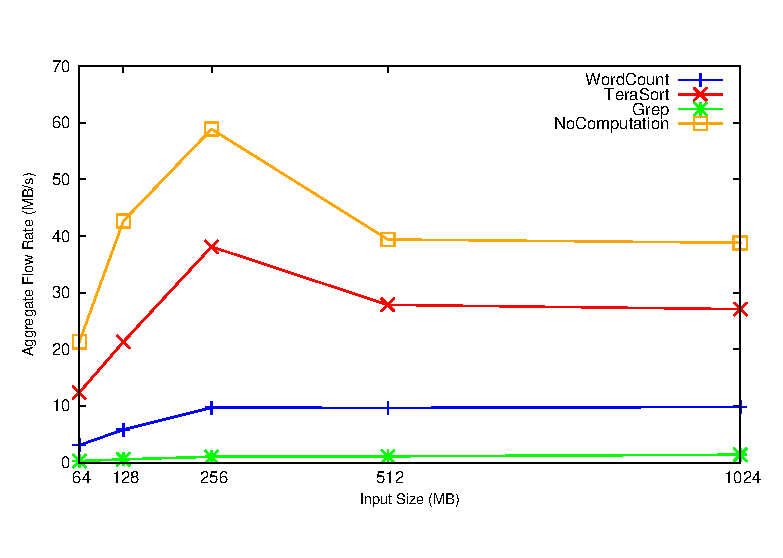
\includegraphics[width=0.8\textwidth]{figures/flow_rate_processing.eps}
    \caption{Estimating flow rate of processing capability.  Increasing the number of concurrent tasks does not necessarily increase the aggregate throughput; instead, it decreases the throughput, especially when the tasks are network intensive.  The computing facility in Cluster 1 has the processing flow capability that is lower than 60MB/s.}
    \label{fig:processing_flow_capability}
\end{figure}


To estimate the flow demand of tasks, we vary input sizes to measure $R^{t}_{in}$ for map tasks, and we fixed the number of reduce tasks to one.
We pick up the flow rate when only one map executes in a computing facility.
This ensures that other tasks would not compete resources with the map task we measure.
$R^{t}_{out}$ of map tasks is set to zero because the output data would be staged and later will be pulled by reduce tasks.

It is more tricky to estimate $R^{t}_{in}$ of reduce tasks because there are multiple sources of flow supply (the shuffle phase contains many-to-many communication \cite{ChowdhuryM2011_Orchestra}) and a reduce task can start even before all map tasks complete.
Moreover, the input size can also affect the flow demand.
These cases can make the elapse time of reduce tasks longer and would affect the accuracy of estimating flow demand.
To eliminate the impact, we use only one reducer in our estimation and we calculate the real flow demand in runtime, which is described as in Section \ref{sec:min_cost_flow}.

\begin{table}[htp]
\caption{Estimated flow capability of facilities. Cluster 1 is powerful than Cluster 2 and their detailed configurations are describe in Section \ref{sec:evaluation}}
\begin{center}
\begin{tabular}{ | l || c | c | }
\hline
Facility Type & $R^{c}_{p}$ & $R^{s}_{out}$ \\
\hline
Cluster 1 & 60 MB/s & 85 MB/s \\
\hline
Cluster 2 & 20 MB/s & 85 MB/s \\
\hline
\end{tabular}
\end{center}
\label{tab:flow_capability}
\end{table}

\begin{table}[htp]
\caption{Estimating flow demand of tasks.  Only one map and  one reduce execute at a time to ensure the estimation accuracy. Lower flow rate suggests it is a CPU-intensive task and it is likely to be a network-inattentive task if flow rate is hight.  Terasort requires high demand of bandwidth and Grep requires more computing power (with search pattern .*kinmen.*) }
\begin{center}
\begin{tabular}{ | l || c | c | c | c | c | }
\hline
& \multicolumn{2}{ |c| }{Cluster 1} & \multicolumn{2}{|c|}{Cluster 2} & \\
\hline
Job Type & $r^{t}_{in} (map)$ & $r^{t}_{in} (reduce) $ & $r^{t}_{in} (map)$ & $r^{t}_{in} (reduce) $ & $in/out \; ratio$\\
\hline
WordCount & 3.04 MB/s & 7.63 MB/s &  3.20 MB/s & 7.63 MB/s & 20\% \\
\hline
Terasort & 9.14 MB/s & 13.31 MB/s & 12.8 MB/s & 22.18 MB/s & 100\% \\
\hline
Grep & 0.23 MB/s & very small & 0.27 MB/s & very small & very small \\
\hline
NoComputation & 16.0 MB/s & 0 MB/S & 21.3 MB/s & 0 MB/S & 0\% \\
\hline
\end{tabular}
\end{center}
\label{tab:flow_demand}
\end{table}
